\documentclass[12pt]{article}
\usepackage[utf8]{inputenc}
\usepackage{amsmath,amssymb,latexsym}
\usepackage{enumerate,comment}
\usepackage{graphicx}
\usepackage[spanish]{babel}
\usepackage{xypic}
\usepackage{graphicx}

\textheight=25cm \textwidth=18cm \topmargin=-2cm \oddsidemargin=-1cm

\newcommand{\abs}[1]{\left\vert#1\right\vert}
\newcommand{\norm}[1]{\left\Vert#1\right\Vert}

\newcommand{\Co}{\mathfrak C}
\newcommand{\diag}{\mathrm{diag}}
\newcommand{\Ext}{\mathrm{ext}}
\newcommand{\F}{\mathfrak F}
\newcommand{\h}{\mathrm h}
\newcommand{\Int}{\mathrm{int}}
\newcommand{\n}{\mathfrak{n}}
\newcommand{\N}{\mathbb N}
\newcommand{\Q}{\mathbb Q}
\newcommand{\R}{\mathbb R}
\newcommand{\US}{\mathbb{S}^2}
\newcommand{\x}{\mathrm x}
\newcommand{\xk}{(\x_k)_{k\in \N}}
\newcommand{\y}{\mathrm y}
\newcommand{\z}{\mathrm z}
\newcommand{\Z}{\mathbb Z}

\newcommand{\eps}{\varepsilon}
\newcommand{\lbil}{\left <}
\newcommand{\rbil}{\right >}
\newcommand{\To}{\longrightarrow}
\newcommand{\mTo}{\longmapsto}

\begin{document}

\pagestyle{empty}
\begin{center}
{\textsc{Cálculo Diferencial e Integral III} \\
\medskip 
\large{Ejercicios I - 1 \\
Luis David Uicab Martínez \\
(El espacio euclidiano de dimensión $n$)}}
\end{center}
\bigskip

En general, $\Omega,\Delta,...$ serán subconjuntos del espacio euclidiano $\R^n$.

\begin{enumerate}

\item 
\begin{enumerate}[(1)]
\item Verifica que las funciones
\[ 
\norm{\x}_{\max} := \max\{\abs{x_1},\ldots,\abs{x_n}\} \quad \text{y}\quad 
\norm{\x}_1 := \abs{x_1} + \cdots + \abs{x_n} 
\]
satisfacen las propiedades de una norma en $\R^n$.
\item Describe las bolas unitarias en $\R^2$ con respecto a las normas $\norm{\x}_{\max}$ y $\norm{\x}_1$. 
\end{enumerate}

\textbf{Solución.}
\begin{enumerate}[(1)]
    \item Empezaremos probando que $\norm{\x}_{\max}$ es norma. Tomemos $k \in \{1,...,n\}$ tal que \\
    $\abs{x_k}=\max\{\abs{x_1},\ldots,\abs{x_n}\}$. Así, $\norm{\x}_{\max}=\abs{x_k} \geq 0$. Por otra parte, notemos que
    \begin{equation*}
        \norm{\x}_{\max}=0 \iff \abs{x_k}=0,
    \end{equation*}
    con lo que, añadiendo propiedades del máximo, obtenemos
    \begin{align*}
            0 \leq \abs{x_i} \leq \abs{x_k} = 0, \quad \forall i\in \{1,...,n\} &\iff \abs{x_i}=0, \quad \forall i \in \{1,...,n\} \\
            &\iff \x = 0. \tag{1}
    \end{align*}
    Ahora tomemos $\lambda \in \R$. Luego, puesto que $\abs{\lambda} \geq 0$ (y recordando que $x_k$ es un máximo), se tiene que
    \begin{align*}
        \abs{\lambda}\abs{x_i} \leq \abs{\lambda}\abs{x_k}, \quad \forall i\in \{1,...,n\} &\implies \abs{\lambda x_i} \leq \abs{\lambda x_k}, \quad \forall i\in \{1,...,n\} \\
        &\implies \abs{\lambda x_k}=\max\{\abs{x_1},\ldots,\abs{x_n}\} \\
        &\implies \norm{\lambda \x}_{\max}=\abs{\lambda x_k},
    \end{align*}
    y en consecuencia,
    \[
    \norm{\lambda \x}_{\max}=\abs{\lambda x_k}=\abs{\lambda}\abs{x_k}=\abs{\lambda}\norm{\x}_{\max}. \tag{2}
    \]
    Definamos $Z=(z_1,\ldots,z_n) \in \R^n$. Sean $k_1,k_2\in \{1,...,n\}$ tales que $\abs{z_{k_1}}=\norm{\z}_{\max}$, y $\abs{x_{k_2}+z_{k_2}}=\norm{\x+\z}_{\max}$. Luego, de las propiedades del
    valor absoluto y del máximo, obtenemos que
    \begin{align*}
        \norm{x+z}_{\max} &= \abs{x_{k_2}+z_{k_2}} \\
        &\leq \abs{x_{k_2}} + \abs{z_{k_2}} \\
        &\leq \abs{x_k} + \abs{z_{k_1}} \\
        &= \norm{\x}_{\max} + \norm{\z}_{\max},
    \end{align*}
    de lo cual,  aunado a $(1)$ y $(2)$ decimos que $\norm{\x}_{\max}$ es una norma en $\R^n$.
    
    
    Respecto a $\norm{\x}_1$, sabemos que de las propiedades del valor absoluto, $\abs{x_i}\geq 0$
    para todo $i$ en $\{1,\dots,n\}$. En consecuencia,
    \[
    \norm{\x}_1 = \sum_{i=1}^{n}\abs{x_i} \geq 0. \tag{3}
    \]
    Para probar que $\norm{\x}_1=0$ si y solo si $\x=0$, procederemos por contradicción. Supongamos que existe $\y=(y_1,\ldots,y_n) \in \R^n$ tal que $\norm{\y}_1=0$, y satisface que existe $k \in \{1,\ldots,n\}$
    con $y_k\neq 0$. En consecuencia, $\abs{y_k}>0$, y por dicha razón, la suma en (3) es estrictamente positiva, lo cual es una contradicción, obteniendo así el resultado. Tomemos $\lambda$ como antes. Así,
    \begin{align*}
        \norm{\lambda\x}_1 &= \sum_{i=1}^{n}\abs{\lambda x_i} \\
        &= \sum_{i=1}^{n}\abs{\lambda}\abs{x_i} \\
        &= \abs{\lambda}\sum_{i=1}^{n}\abs{x_i} \\
        &= \abs{\lambda}\norm{\x}_1.
    \end{align*}
    Nuevamente, tomemos el vector $Z$. Luego, por propiedades del valor absoluto, tenemos que $\abs{x_i+z_i}\leq \abs{x_i}+\abs{z_i}$ para todo $i \in \{1,\ldots,n\}$. De ello, afirmamos que
    \begin{align*}
       \norm{\x-\z}_1 &= \sum_{i=1}^{n}\abs{x_i-z_i} \\
       &\leq \sum_{i=1}^{n}\left(\abs{x_i} + \abs{z_i}\right) \\
       &=\sum_{i=1}^{n}\abs{x_i} + \sum_{i=1}^{n}\abs{z_i} \\
       &=\norm{\x}_1 + \norm{\z}_1,
    \end{align*}
    de lo cual se colige que $\norm{\x}_1$ también es norma de $\R^n$.

    \item Dada la norma $\norm{\x}_{\max}$, tenemos que la bola unitaria en $\R^2$ está descrita como
    \begin{align*}
        B_1(0) &= \left\{\y\in\R^2:\norm{\y}_{\max} < 1 \right\} \\
        &= \left\{(y_1,y_2)\in\R^2:\norm{(y_1,y_2)}_{\max} < 1 \right\} \\
        &= \left\{(y_1,y_2)\in\R^2:\max\{\abs{y_1},\abs{y_2}\} < 1 \right\} \\
        &= \left\{(y_1,y_2)\in\R^2:\max\{\abs{y_1},\abs{y_2}\} < 1 \right\} \\
        &= \left\{(y_1,y_2)\in\R^2:\abs{y_1} < 1,\abs{y_2} < 1 \right\}.
    \end{align*}

    \vspace{5cm}

    \begin{figure}[h]
        \centering
        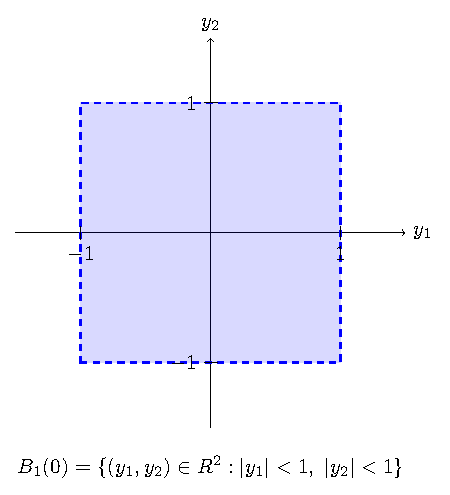
\includegraphics[width=0.4\textwidth]{cuadrado.pdf}
    \end{figure}
    Y finalmente, se tiene que la bola unitaria en $\R^2$ asociada a la norma $\norm{\x}_1$ es
    \begin{align*}
        B_1(0) &= \left\{\y\in\R^2:\norm{\y}_{1}\leq 1 \right\} \\
        &= \left\{(y_1,y_2)\in\R^2:\norm{(y_1,y_2)}_{1}< 1 \right\} \\
        &= \left\{(y_1,y_2)\in\R^2:\abs{y_1}+\abs{y_2}< 1 \right\}. \quad \blacktriangle
    \end{align*}
        \begin{figure}[h]
        \centering
        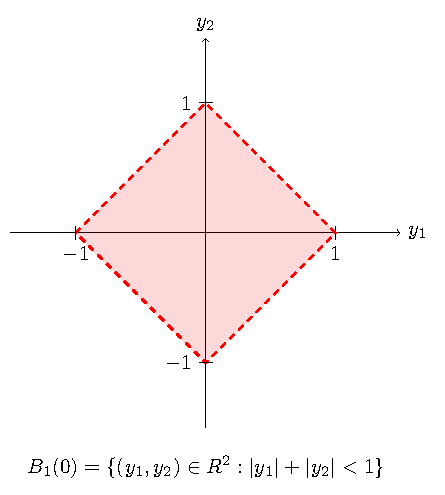
\includegraphics[width=0.4\textwidth]{rombo.pdf}
    \end{figure}
\end{enumerate}

\newpage
\item Demuestra que se cumplen las siguientes desigualdades:
\begin{enumerate}[(1)]
\item $\norm{\x}_{\max}\leq \norm{\x}\leq \sqrt{n}\norm{\x}_{\max}$.
\item $\frac{1}{\sqrt{n}}\norm{\x}_1\leq \norm{\x}\leq \norm{\x}_1$.
\end{enumerate}

\textbf{Demostración.}
\begin{enumerate}[(1)]
    \item Tomemos $k \in \{1,\ldots,n\}$ tal que $\abs{x_k}=\norm{\x}$. Puesto que los cuadrados son números
    no negativos, afirmamos que
    \begin{align*}
        0 \leq \sum_{i\in \{1,\ldots,n\}\setminus \{k\}}x_{i}^2 &\implies x_k^2 \leq x_k^2 + \sum_{i\in \{1,\ldots,n\}\setminus \{k\}}x_{i}^2 \\
        &\implies x_{k}^2 \leq \sum_{i=1}^{n}x_i^2 \\
        &\implies \sqrt{x_{k}^2} \leq \sqrt{\sum_{i=1}^{n}x_i^2} \\
        &\implies \abs{x_{k}} \leq \norm{\x} \\
        &\implies \norm{\x}_{\max} \leq \norm{\x}.
    \end{align*}
    Luego, dada la definición de $\abs{x_k}$, afirmamos que
    \begin{align*}
        \abs{x_i}\leq \abs{x_k}, \quad \forall i \in \{1,\ldots,n\} &\implies  x_i^2\leq  x_k^2, \quad \forall i \in \{1,\ldots,n\}\\
        &\implies \sum_{i=1}^{n}x_i^2 \leq \sum_{i=1}^{n}x_k^2 \\
        &\implies \sum_{i=1}^{n}x_i^2 \leq nx_k^2 \\
        &\implies \sqrt{\sum_{i=1}^{n}x_i^2} \leq \sqrt{nx_k^2} \\
        &\implies \norm{\x} \leq \sqrt{n}\abs{x_k} \\
        &\implies \norm{\x} \leq \sqrt{n}\norm{\x}_{\max},
    \end{align*}
    de lo que se sigue el resultado.
    \item A priori, señalamos que $\abs{x_i}$ para todo $i \in \{1,\ldots,n\}$ cumple que es no negativo. De dicha hipótesis y dada la desigualdad de la media cuadrática-media
    aritmética, deducimos que
    \begin{align*}
        \frac{1}{n}\sum_{i=1}^{n}\abs{x_i} \leq \sqrt{\frac{1}{n}\sum_{i=1}^{n}\abs{x_i}^2} &\implies \frac{1}{n}\sum_{i=1}^{n}\abs{x_i} \leq \frac{1}{\sqrt{n}}\sqrt{\sum_{i=1}^{n}x_i^2}\\
        &\implies \frac{1}{\sqrt{n}}\sum_{i=1}^{n}\abs{x_i} \leq \sqrt{\sum_{i=1}^{n}x_i^2} \\
        &\implies \frac{1}{\sqrt{n}}\norm{\x}_1 \leq \norm{\x}.
    \end{align*}
    Por otra parte, notemos que
    \begin{align*}
        \left(\sum_{i=1}^{n}\abs{x_i}\right)^2 = \sum_{i=1}^{n}x_i^2 + 2\sum_{1\leq j<k\leq n}\abs{x_jx_k} &\implies \sum_{i=1}^{n}x_i^2 \leq \left(\sum_{i=1}^{n}\abs{x_i}\right)^2\\
        &\implies \sqrt{\sum_{i=1}^{n}x_i^2} \leq \sum_{i=1}^{n}\abs{x_i} \\
        &\implies \norm{\x} \leq \norm{\x}_{1},
    \end{align*}
    con lo que damos por concluida la demostración. $\blacksquare$
\end{enumerate}

\newpage
\item Describe el interior de
\[ \Omega = \{ (x,y,z)\in \R^3 : 0\leq x < 1, y^2+z^2\leq 1\}. \]
\textbf{Solución.} \\
Sea $\Delta=\{(x,y,z)\in \R^3 : 0 < x < 1, y^2+z^2<1\}$. Probaremos que dicho conjunto es el interior de $\Omega$. Tomemos $u=(u_1,u_2,u_3)\in \Delta$ arbitrario. Definamos $r=\min\left\{1,1-u_1,1-\sqrt{u_2^2+u_3^2}\right\}$. Tomemos ahora un punto
$v=(v_1,v_2,v_3) \in B_{r}(u)$ arbitrario. Al estar $v$ en dicha bola, se cumple que
\begin{align*}
    \norm{u-v} < r &\iff \sqrt{(u_1-v_1)^2+(u_2-v_2)^2+(u_3-v_3)^2}<r \\
    &\iff (u_1-v_1)^2+(u_2-v_2)^2+(u_3-v_3)^2 < r^2. \tag{1}
\end{align*}
En particular, se cumple que
\begin{align*}
    (u_1-v_1)^2 < r^2 &\implies |u_1-v_1| < r \\
    &\implies |v_1-u_1| < u_1, \quad |v_1-u_1|<1-u_1 \\
    &\implies -u_1 < v_1 - u_1 < u_1, \quad u_1 - 1 < v_1 - u_1 < 1 - u_1 \\
    &\implies 0 < v_1 < 2u_1, \quad 2u_1 - 1 < v_1 < 1 \\
    &\implies 0 < v_1 < 1. \tag{2}
\end{align*}
Por otra parte, definiendo $\x=(u_2,u_3),\y=(v_2,v_3)$, de la desigualdad en $(1)$ decimos que
\begin{align*}
    (u_2-v_2)^2 + (u_3-v_3)^2 < r^2 &\implies \sqrt{(u_2-v_2)^2 + (u_3-v_3)^2} < 1-\sqrt{u_2^2+u_3^2} \\
    &\implies \norm{\x-\y} < 1 - \norm{\x} \\
    &\implies \norm{\x-\y} + \norm{\x} < 1.
\end{align*}
Notése que de la desigualdad del triángulo, tenemos la desigualdad
\[
\norm{\y} = \norm{\y + \x - \x} \leq \norm{\y-\x} + \norm{\x} = \norm{\x-\y} + \norm{\x},
\]
de lo que se sigue $\sqrt{v_2^2+v_3^2} = \norm{\y} < 1$, y en adición, $v_2^2+v_3^2 < 1$. Luego, por lo dicho en $(2)$,
se tiene que $v \in \Omega$, y por lo tanto $u \in \text{int}(\Omega)$, concluyendo así que $\Delta \subset \text{int}(\Omega)$. Tomemos ahora $u=(u_1,u_2,u_3) \in \text{int}(\Omega)$. Dado que $\text{int}(\Omega)\subset \Omega$, se tiene que
$0\leq u_1 < 1$ y $u_2^2+u_3^2 \leq 1$. Supongamos que $u_1 = 0$. Sea $r > 0$ arbitrario y $v=(-\varepsilon,u_2,u_3)$ con $0<\varepsilon<r$. Notemos que
\[
\norm{u-v}=\sqrt{(0-\varepsilon)^2+(u_2-u_2)^2+(u_3-u_3)^2} = \varepsilon < r.
\]
Luego, $v \in B_r(u)$. Sin embargo, $v \notin \Omega$, de lo que se sigue $u \notin \text{int}(\Omega)$, lo cual es una contradicción y por lo tanto, $u_1 > 0$. Veamos que pasa si $u_2^2+u_3^2=1$. \\ Sea $r > 0$ arbitrario y
$v=(u_1,u_2+\varepsilon_1,u_3+\varepsilon_2+u_3)$,
donde 
\[
\varepsilon_1=
\begin{cases}
    -\varepsilon, u_2 < 0 \\
    \varepsilon, u_2 \geq 0
\end{cases}  \text{y} \quad 
\varepsilon_2=
\begin{cases}
    -\varepsilon, u_3 < 0 \\
    \varepsilon, u_3 \geq 0
\end{cases} \text{para algún } 0 < \varepsilon < r/\sqrt{2}.
\]
De esta forma
\begin{align*}
    \norm{u-v} &= \sqrt{(u_1-u_1)^2+(u_2-(u_2+\varepsilon_1))^2 + (u_3-(u_3+\varepsilon_3))^2} \\
    &= \sqrt{\varepsilon_1^2 + \varepsilon_2^2} \\
    &= \sqrt{2\varepsilon^2} \\
    &= \sqrt{2}\varepsilon \\
    &< r.
\end{align*}
Así, $v \in B_r(u)$. Sin embargo, notemos que por las definiciones de $\varepsilon_1$ y $\varepsilon_2$, se tiene que
\begin{align*}
    \abs{u_2} < \abs{u_2+\varepsilon_1}, \quad \abs{u_3}<\abs{u_3+\varepsilon_2} &\implies u_2^2 < (u_2+\varepsilon_1)^2, \quad u_3^2 < (u_3+\varepsilon_2)^2 \\
    &\implies 1= u_2^2 + u_3^2 < (u_2+\varepsilon_1)^2 + (u_3+\varepsilon_2)^2
    &\implies u \notin \Omega,
\end{align*}
lo cual es una contradicción, de lo que deducimos, $v_2^2+v_3^2<1$. Así, $v \in \Delta$, y por lo tanto $\text{int}(\Omega)\subset \Delta$, lo que aunado a la contención
previamente hecha, nos hace concluir que $\Delta=\text{int}(\Omega)$. $\blacktriangle$


\newpage
\item Encuentra la frontera de 
\[ \Omega = \{ (x,y)\in \R^2 : x^2 - y^2 > 1 \}. \]
\textbf{Solución.} \\
Definimos $\Delta = \{(x,y)\in \R^2:x^2-y^2=1\}$. De la definición de $\Omega$, sabemos que $\Omega^c=\{(x,y)\in \R^2:x^2-y^2\leq 1\}$. Tomemos $u=(u_1,u_1) \in \Delta$ y $r>0$ arbitrarios. Definimos
\[
r_1=
\begin{cases}
    -r/2, u_1 < 0 \\
     r/2, u_1 \geq 0
\end{cases}
\]
Notemos que $v=(u_1+r_1,u_2) \in B_r(u)$. Luego, tenemos que
\begin{align*}
    \abs{u_1} < \abs{u_1+r_1} &\implies u_1^2 < (u_1+r_1)^2 \\
    &\implies 1 = u_1^2 - u_2^2 < (u_1+r_1^2) - u_2^2 \\
    &\implies v \in \Omega \\
    &\implies B_r(u)\cap \Omega \neq \varnothing.
\end{align*}
Luego, como $u \in B_r(u)$ y $u \in \Omega^c$, se sigue que $B_r(u)\cap \Omega \neq \varnothing$ y en adición, $u \in \partial\Omega$. Así, $\Delta \subset \partial\Omega$.
\newpage
\item Decir si las siguientes propiedades son ciertas. Prueba tu respuesta.
\begin{enumerate}[(1)]
\item $\Int(\Omega\cup \Delta) = \Int(\Omega)\cup \Int(\Delta),\; \Int(\Omega\cap \Delta) = \Int(\Omega)\cap \Int(\Delta)$.
\item $\Ext(\Omega\cup \Delta) = \Ext(\Omega)\cup \Ext(\Delta),\; \Ext(\Omega\cap \Delta) = \Ext(\Omega)\cap \Ext(\Delta)$.
\end{enumerate}
\textbf{Solución.}
\begin{enumerate}[(a)]
    \item Falso. Sea $\Omega=(-\infty,-1]\cup[1,\infty)$ y $\Delta=[-1,1]$. Así, $\text{int}(\Omega)=(-\infty,-1)\cup(1,\infty)$ e $\text{int}(\Delta)=(-1,1)$. En consecuencia
    \begin{align*}
        \text{int}(\Omega)\cup \text{int}(\Delta) &= \R\setminus \{-1,1\} \\
        &\neq \R \\
        &=\text{int}(\R) \\
        &=\text{int}(\Omega\cup \Delta).
    \end{align*}
    \item Verdadero. Sea $x \in \text{int}(\Omega\cap\Delta)$. Así, se cumple que existe $r>0$ tal que $B_r(x)\subset \Omega \cap \Delta$. En particular, afirmamos que $B_r(x)\subset \Omega$ y
    $B_r(x)\subset \Delta$. En consecuencia, $x \in \text{int}(\Omega)$ y $x \in \text{int}(\Delta)$. Se sigue que $x \in \text{int}(\Omega)\cap\text{int}(\Delta)$, y por lo tanto,
    $\text{int}(\Omega\cap\Delta) \subset \text{int}(\Omega)\cap\text{int}(\Delta)$. Tomemos ahora $x \in \text{int}(\Omega)\cap\text{int}(\Delta)$. De dicha pertenencia, se sigue que existen $r_1.r_2>0$
    tales que $B_{r_1}(x)\subset \Omega$ y $B_{r_2}(x)\subset \Delta$. Tomése $r=\min\{r_1,r_2\}$. Así, se sigue que $B_{r}(x)\subset \Omega$ y $B_r(x)\subset \Delta$. Luego, $B_{r}(x)\subset \Omega \cap \Delta$,
    y en adición $x \in \text{int}(\Omega\cap \Delta)$, de lo que se sigue $\text{int}(\Omega)\cap\text{int}(\Delta)\subset \text{int}(\Omega\cap \Delta)$. De ello y por la contención ya antes dicha, concluimos que
    $\text{int}(\Omega)\cap\text{int}(\Delta)=\text{int}(\Omega\cap \Delta)$.
    \item Falso. De la igualdad del inciso (b) de este ejercicio decimos que
    \begin{align*}
        \text{ext}(\Omega\cup \Delta) &= \text{int}((\Omega\cup\Delta)^c)\\
        &= \text{int}(\Omega^c\cap \Delta^c) \\
        &= \text{int}(\Omega^c)\cap \text{int}(\Delta^c) \\
        &= \text{ext}(\Omega)\cap \text{ext}(\Delta) \\
        &\neq \text{ext}(\Omega)\cup \text{ext}(\Delta). \tag{1}
    \end{align*}
    \item Falso. Se sigue de la igualdades mencionadas en $(1)$. $\blacktriangle$
\end{enumerate}


\newpage
\item Decir si las siguientes propiedades son ciertas. Prueba tu respuesta.
\begin{enumerate}[(1)]
\item $\partial(\Omega\cup \Delta) = \partial \Omega\cup \partial \Delta,\; 
\partial(\Omega\cap \Delta) = \partial \Omega\cap \partial \Delta$.
\item Si $\Omega\subset \Delta$ entonces $\Int(\Omega)\subset \Int(\Delta),\; \Ext(\Omega)\subset \Ext(\Delta),\; \partial \Omega\subset \partial \Delta$.
\end{enumerate}
\textbf{Solución.}
\begin{enumerate}[(a)]
    \item Falso. Si $\Omega=[0,1],\Delta=[0,2]$, entonces $\partial\Omega=\{0,1\}$ y $\partial\Delta=\{0,2\}$. Luego, $\partial\Omega\cup\partial\Delta=\{0,1,2\}$.
    Por otra parte, $\Omega \cup \Delta=[0,2]$. Así, $\partial(\Omega\cup\Delta)=\{0,2\}\neq \partial\Omega\cup\partial\Delta$, de lo que se sigue el resultado.
    \item Falso. Si $\Omega=[0,1),\Delta=[1,2]$, entonces $\partial\Omega=\{0,1\}$ y $\partial\Delta=\{1,2\}$. De ello, $\partial\Omega\cap\partial\Delta=\{1\}$. Finalmente,
    $\partial(\Omega\cap\Delta)=\partial(\varnothing)=\varnothing\neq \partial\Omega\cap\partial\Delta$, obteniendo así el resultado.
    \item Verdadero. Sea $x \in \text{int}\Omega$ arbitrario. Por lo tanto existe $r>0$ tal que $B_r(x)\subset \Omega$. Puesto que $\Omega \subset \Delta$, se tiene que $B_r(x)\subset \Delta$,
    y en adición, $x \in \text{int}(\Delta)$, de lo que concluimos $\text{int}(\Omega)\subset \text{int}(\Delta)$.
    \item Falso. Si $\Omega=[0,1],\Delta=[0,2]$ (nótese $\Omega\subset \Delta$), entonces $\text{ext}(\Omega)=(-\infty,0)\cup (1,\infty)$ y $\text{ext}\Delta=(-\infty,0)\cup (2,\infty)$, dónde hacemos notar que
    $(-\infty,0)\cup (2,\infty)\subset (-\infty,0)\cup (1,\infty)$, de lo que se sigue el resultado.
    \item Falso. Si $\Omega=[0,1],\Delta=[0,2]$, entonces $\partial\Omega=\{0,1\}$ y $\partial\Omega=\{0,2\}$ donde $\{0,1\}\nsubseteq \{0,2\}$ obteniendo así el resultado. $\blacktriangle$
\end{enumerate}

\newpage
\item Define la \emph{suma} de $\Omega$ y $\Delta$ como
\[ \Omega + \Delta := \{ \x+\y\in \R^n : \x\in \Omega, \y\in \Delta \}. \]
Demuestra que si $\Omega$ o $\Delta$ es abierto, $\Omega + \Delta$ es abierto. \\
\textbf{Demostración.} \\
Sin pérdida de generalidad, supongamos que $\Omega$ es abierto. Tomemos $z \in \Omega+\Delta$ arbitrario. Así, existen $x \in \Omega$ y $y \in \Delta$
tales que $z=x+y$. Puesto que $\Omega$ es abierto, existe $r>0$ tal que $B_r(z)\subset \Omega$. Luego, tomemos $v \in B_r(z)$ arbitrario. Así, se tiene que
\begin{align*}
    r &> \norm{z-v} \\
    &= \norm{v-z} \\
    &= \norm{(v-y)-x},
\end{align*}
de lo que afirmamos, $v-y \in B_r(x)\subset \Omega$. Como $y\in \Delta$, se sigue que $v=(v-y)+v \in \Omega + \Delta$. En consecuencia, $B_r(z)\subset \Omega+\Delta$,
de lo que concluimos, $\Omega+\Delta$ es un abierto. $\blacksquare$

\newpage
\item Encuentra la cerradura de 
\[ \Omega = \{ (x,y)\in \R^2 : x > y^2 \}. \]
\textbf{Solución.} Sea $\Delta=\{(x,y)\in \R^2:x=y^2\}$. Tomemos $v=(v_1,v_2) \in \Delta$ y $r>0$ arbitrarios. Hacemos ver que los valores de la coordenada en $x$
son estrictamente no negativo, pues son el cuadrado de las coordenadas en $y$. Definamos $\varepsilon_1=r/2$.
Así, notemos que $v'=(v_1+\varepsilon_1,v_2) \in B_r(u)$. Luego, afirmamos que $v_1<v_1+\varepsilon_1$. Como por definición, $v$ cumple que
$v_1=v_2^2$, en particular, $v_2^2 < v_1+\varepsilon_1$ de lo que se sigue, $v'\in \Omega$. Así, $B_r(v)\cap \Omega \neq \varnothing$. Por otra parte, notemos que $v \in \Omega^c$,
de lo que se sigue, $B_r(v)\cap \Omega \neq \varnothing$. En adición, $v \in \partial\Omega$, y por lo tanto $\Delta \subset \partial\Omega.$

\newpage
\item Prueba que si $\Omega$ es cerrado entonces 
$\Int(\partial \Omega)=\emptyset$. \\
\textbf{Demostración.} \\
Procederemos por contradicción y supondremos que existe $x_0 \in \partial\Omega$ tal que para algún $r>0$, $B_r(x_0)\subset \partial\Omega.$ Puesto que
$x_0 \in \partial\Omega$, se sigue que $B_r(x_0)\cap (\R^n\setminus \Omega)\neq \varnothing$, es decir, existe $x_1 \in B_r(x_0)$ tal que $x_1 \in \R^2\setminus \Omega$. Como además,
$\Omega$ es cerrrado, afirmamos que $\partial\Omega \subset \Omega$ y en particular, $B_r(x_0)\subset \Omega$. De esto último, podemos afirmar que $x_1 \in \Omega$, pero esto es una contradicción,
puesto que dicho punto pertenecía al complemento, de lo que se sigue el resultado. $\blacksquare$

\item Supongamos que $a_1,\ldots,a_n,b_1,\ldots,b_n\in \R^n$ son tales que $a_j<b_j$ para toda $j=1,\ldots,n$. Hemos definimos el rectángulo cerrado (abierto) por
\[ R = [a_1,b_1]\times \cdots\times [a_n,b_n], \]
o bien,
\[ R = (a_1,b_1)\times \cdots\times (a_n,b_n). \]
En cualquier caso, la \textsf{diagonal} de $R$ se define por:
\[ \diag(R) := \norm{(b_1,\ldots,b_n) - (a_1,\ldots,a_n)}. \]
Prueba que todo rectángulo cerrado $R$ es un subconjunto cerrado, acotado y convexo de $\R^n$. 
\textbf{Demostración.} \\ 
Definamos $r_0=\max\{\abs{a_1},\ldots,\abs{a_n},\abs{b_1},\ldots,\abs{b_n}\}$. Sea $R'=[-r_0,r_0]^n$ (producto cruz consigo mismo n-veces). Puesto que
para $i\in \{1,...,n\}$ arbitrario se cumple que $-r_0\leq a_i,b_i \leq r_0$, se tiene que $[a_i,b_i]\subset [-r_0,r_0]$ para toda $i \in \{1,...,n\}$, y en consecuencia,
$R\subset R'$, con lo que afirmamos, $R$ es acotado. \\ Tomemos ahora $u=(u_1,...,u_n) \in R^c$ arbitrario. Así, existe $t \in \{1,...,n\}$ tal que $u_t<a_t$ o $b_t<u_t$. Supongamos que $b_t<u_t$ (el
caso para $u_t<a_t$ es análogo). Sea $r=u_t-b_t>0$. Tomemos $v=(v_1,...,v_n) \in B_r(u)$ arbitrario. De dicha pertenencia, afirmamos que
\begin{align*}
    u_t-b_t > \norm{u-v} &\implies u_t-b_t > \sqrt{\sum_{i=1}^{n}(u_i-v_i)^2} \\
    &\implies  (u_t-b_t)^2 > \sum_{i=1}^{n}(u_i-v_i)^2 \\
    &\implies (u_t-b_t)^2 > (u_t-v_t)^2 \\
    &\implies u_t-b_t=\abs{u_t-b_t} > \abs{u_t-v_t} \geq u_t-v_t \\
    &\implies v_t > b_t > u_t \\
    &\implies v \in R^c.
\end{align*}
Puesto que $v$ fue arbitrario, tenemos que $B_r(u)\subset R^c$, y en consecuencia, $R^c$ es abierto. Así, $(R^c)^c=R$ es cerrado. \\ Resta probar que $R$ es conexo. Tomemos $x=(x_1,...,x_n),y=(y_1,...,y_n)\in R$
arbitarios. Queremos probar que
\begin{align*}
    [x,y]=\{tx+(1-t)y:0\leq t \leq 1\}\subset R.
\end{align*}
Dado que $x,y\in R$, se sigue que $a_i\leq x_i,y_i \leq b_i$ para toda $i \in \{1,..,n\}$. En consecuencia, para $0\leq t \leq 1$,
\[
a_it\leq x_it,\quad (1-t)a_i\leq (1-t)y_i, \quad x_it\leq y_it, \quad (1-t)y_i \leq (1-t)y_i,
\]
de lo que se sigue
\[
a_i=a_it+(1-t)a_i \leq x_it+(1-t)y_i \leq b_it + (1-t)b_i = b_i, \quad \forall i\in \{1,...,n\}.
\]
Así, afirmamos que $tx+(1-t)y \in R,$ para $t\in [0,1]$ arbitrario, con lo que concluimos, $[x,y]\subset R$ y por lo tanto $R$ es conexo. $\blacksquare$
\end{enumerate}

\end{document}
